% For VIM to recognize the document syntax \begin{document} and \end{document}
% - However, the compilation will fail!! So don't forget to comment the
%   directives before compiling!!'
%
%\begin{document}
%
% CHAPTER - Introduction -------------------------
\chapter{Introduction}%
\label{ch:introduction}
The present work illustrates the application of the two first stages of the Waterfall methodology
--- Analysis and Design --- to develop a \gls{tv} remote control. This type of project
begins with the establishment of a contract between the client (Samsung company)
and the project team, clearly defining the problem statement and deriving the
product requirements and constraints associated to the project. It should be
noted, however, that both roles are played out by the authors.
A market
research is performed to gain more insight over this market and the
product placement, and the product overall characteristics.

In the analysis
phase, the product requirements are derived --- defining the client expectations
for the product --- as well as the project constraints --- what the environments
limits about the product. Finally, the theoretical foundations are outlined,
providing the basic technical knowledge to undertake the project.

In the design phase, the product development starts, specifying the system in
terms of hardware and software and its associated interfaces, the error handling
required, and the design verification.
%
  \vspace{-5mm}
%  
\section{Problem statement}
\label{sec:prob-stat}
The first step of the project is to clearly define the problem, as a result of
the contract established between the client and the project team, yielding, in
this case, the following project statement:

``Design a remote control with three buttons that can
remotely control the television (TV). It should be very
light, powered by batteries and controls your TV via an
infrared emitter. The TV has a built-in infrared receiver. A
button on the remote control switches the TV on/off and
will be labeled with the word "Power". The other two
buttons are used to scroll up/down and select the available
channels and they are labeled with the arrows up/down.''
%
  \vspace{-5mm}
%  
\section{Market research}
\label{sec:market-research}
A TV remote is a device which is used to operate a television from
distance in a wireless mode. It also makes the TV usage simpler, more user friendly with its suggestive buttons. These buttons control functions such as power, volume, channel switch and various other features.

TV remotes are composed by the TV remote Shell,
the TV remote membrane, one LED and a data acquisition \& Infrared emitter PCB,
as illustrated in Fig.~\ref{fig:remotemat}. The unit cost of universal TV remotes is about 3 to 5 EUR.
%
% Remote material (side by side)
\begin{figure}[htb!]
  \centering
  %
  \begin{subfigure}{.4\textwidth}
  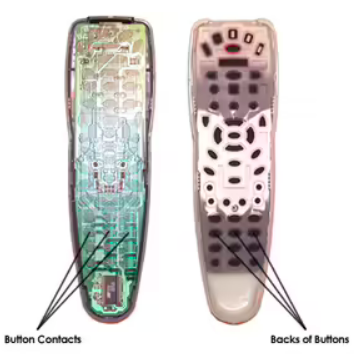
\includegraphics[width=\textwidth]{img/remotematerial1.png}%
  %\caption{KUKA's original position}%
  %\label{fig:ptp-test-orig}
\end{subfigure}
%
  \begin{subfigure}{.4\textwidth}
    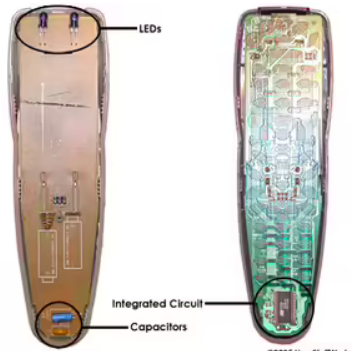
\includegraphics[width=\textwidth]{img/remotematerial2.png}%
%  \caption{KUKA's final position}%
%  \label{fig:ptp-test-final}
\end{subfigure}
%
  \caption{TV Remote control bill of materials, withdrawn from~\cite{remotematerial}}%
  \label{fig:remotemat}
\end{figure}

As can be seen in Fig.~\ref{fig:tvsells}, the amount of televisions sold per
year is about 200 million per year, with a tendency to increase over the next
years. Thus, at least the same amount of TV remotes sells is expected, as each
new TV requires one remote control, but it is expected to be exceeded due to TV
remote replacement arising from its malfunctioning or bad usage.
%
\begin{figure}[htb!]
\centering
    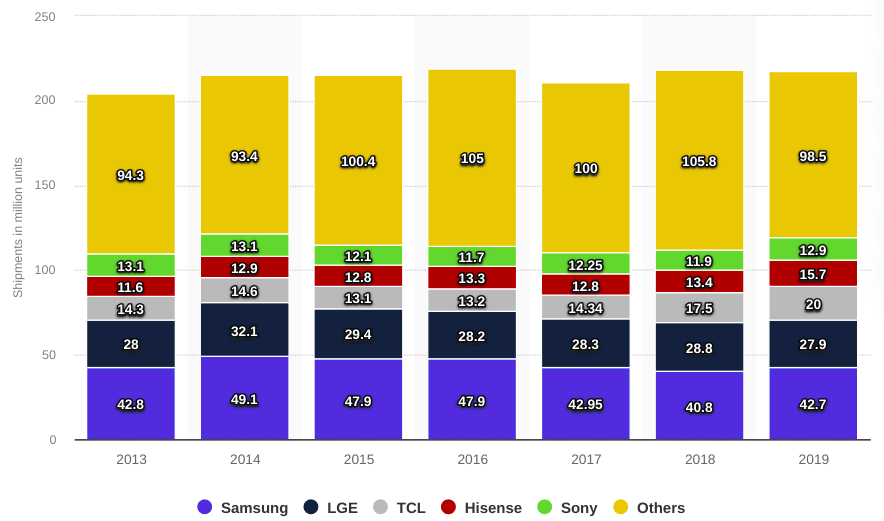
\includegraphics[width=0.7\columnwidth]{./img/tvsellings.png}
  \caption{Global LCD TV unit shipments from 2015 to 2019, by vendor (in
    millions), withdrawn from~\cite{tvsellings}}%
\label{fig:tvsells}
\end{figure}
%
%%% Local Variables:
%%% mode: latex
%%% TeX-master: "../../dissertation"
%%% End:
